\chapter{Технологический раздел}

\section{Выбор  языка программирования и среды разработки}
Для реализации загружаемого модуля был выбран язык С. 
Операционная система Linux позволяет писать загружаемые модули ядра на Rust и на C. 
Rust непопулярен и ещё только развивается и не обладает достаточным количеством документации.
Для реализации клиента был выбран протокол telnet, который имеется в любой современной ОС.
В качестве среды разработки выбран VS Code.

%\newpage
\section{Перехват функций}
В листинге \ref{ftracehook} представлена структура, которая описывает любую перехватываемую функцию.
\begin{lstlisting}[language=c++,,escapeinside={(@}{@)},caption={ftrace\_hook},label={ftracehook}]
	/**
	* struct ftrace_hook - описывает перехватываемую функцию
	* @name:       имя перехватываемой функции
	* @function:   адрес функции-обёртки, которая будет вызываться вместо
	*              перехваченной функции
	* @original:   указатель на место, куда следует записать адрес
	*              перехватываемой функции, заполняется при установке
	* @address:    адрес перехватываемой функции, выясняется при установке
	* @ops:        служебная информация ftrace, инициализируется нулями,
	*              при установке перехвата будет доинициализирована
	*/
	struct ftrace_hook {
		const char *name;
		void *function;
		void *original;
		unsigned long address;
		struct ftrace_ops ops;
	};
\end{lstlisting}

Пользователю необходимо заполнить только первые три поля: name, function, original. Остальные поля считаются деталью реализации. Описание всех перехватываемых функций можно собрать в массив и использовать макросы, чтобы повысить компактность кода, как показано в листинге \ref{ftracehookdefine}.

\newpage
\begin{lstlisting}[language=c++,,escapeinside={(@}{@)},caption={ftrace\_hook define},label={ftracehookdefine}]
	#define HOOK(_name, _function, _original)   \
	{                                       	\
		.name = (_name),                    	\
		.function = (_function),            	\
		.original = (_original),            	\
	}
	static struct ftrace_hook hooked_functions[] = {
		HOOK("sys_clone",   fh_sys_clone,   &real_sys_clone),
	};
\end{lstlisting}

Сигнатуры функций должны совпадать один к одному. Без этого, очевидно, аргументы будут переданы неправильно и всё пойдёт под откос. Для перехвата системных вызовов это важно в меньшей степени, так как их обработчики очень стабильные и для эффективности аргументы принимают в том же порядке, что и сами системные вызовы.

\subsection{Инициализация ftrace}
Для начала нам потребуется найти и сохранить адрес функции, которую мы будем перехватывать. Ftrace позволяет трассировать функции по имени, но нам всё равно надо знать адрес оригинальной функции, чтобы вызывать её.

Добыть адрес можно с помощью kallsyms — списка всех символов в ядре. В этот список входят все символы, не только экспортируемые для модулей. Получение адреса перехватываемой функции показано в листинге \ref{l3}:
\begin{lstlisting}[language=c++,,escapeinside={(@}{@)},caption={resolve\_hook\_address},label={l3}]
	static int resolve_hook_address(struct ftrace_hook *hook)
	{
		hook->address = kallsyms_lookup_name(hook->name);
		if (!hook->address) {
			pr_debug("unresolved symbol: %s\n", hook->name);
			return -ENOENT;
		}
		*((unsigned long*) hook->original) = hook->address;
		return 0;
	}
\end{lstlisting}

Дальше необходимо инициализировать структуру ftrace\_ops. В ней обязательным полем является только func, указывающая на коллбек, но, кроме этого необходимо установить некоторые важные флаги (листинг \ref{l4}).
\newpage
\begin{lstlisting}[language=c++,,escapeinside={(@}{@)},caption={fh\_install\_hook},label={l4}]
	int fh_install_hook(struct ftrace_hook *hook)
	{
		int err = resolve_hook_address(hook);
		if (err)
		return err;
		
		hook->ops.func = fh_ftrace_thunk;
		hook->ops.flags = FTRACE_OPS_FL_SAVE_REGS | FTRACE_OPS_FL_IPMODIFY;
		
		err = ftrace_set_filter_ip(&hook->ops, hook->address, 0, 0);
		if (err) {
			pr_debug("ftrace_set_filter_ip() failed: %d\n", err);
			return err;
		}
		
		err = register_ftrace_function(&hook->ops);
		if (err) {
			pr_debug("register_ftrace_function() failed: %d\n", err);
			ftrace_set_filter_ip(&hook->ops, hook->address, 1, 0);
			return err;
		}
		
		return 0;
	}
\end{lstlisting}

Выключается перехват аналогично, только в обратном порядке (листинг \ref{l5}).
\begin{lstlisting}[language=c++,,escapeinside={(@}{@)},caption={fh\_remove\_hook}, label={l5}]
	void fh_remove_hook(struct ftrace_hook *hook)
	{
		int err = unregister_ftrace_function(&hook->ops);
		if (err) {
			pr_debug("unregister_ftrace_function() failed: %d\n", err);
		}
		
		err = ftrace_set_filter_ip(&hook->ops, hook->address, 1, 0);
		if (err) {
			pr_debug("ftrace_set_filter_ip() failed: %d\n", err);
		}
	}
\end{lstlisting}

После завершения вызова unregister\_ftrace\_function() гарантируется отсутствие активаций установленного коллбека в системе. Поэтому модно выгрузить модуль-перехватчик, не опасаясь, что в системе ещё выполняются функции.

\subsection{Выполнение перехвата функций}

Ftrace позволяет изменять состояние регистров после выхода из коллбека. Изменяя регистр $RIP$ (указатель на следующую исполняемую инструкцию) мы изменяются инструкции, которые исполняет процессор — то есть можно заставить его выполнить безусловный переход из текущей функции в нашу. Таким образом перехватывается управление. Коллбек для ftrace показан в листинге \ref{l6}:
\begin{lstlisting}[language=c++,,escapeinside={(@}{@)},caption={fh\_remove\_hook},label={l6}]
	static void notrace fh_ftrace_thunk(unsigned long ip, 
	unsigned long parent_ip, struct ftrace_ops *ops, 
	struct pt_regs *regs)
	{
		struct ftrace_hook *hook = container_of(ops, struct ftrace_hook, ops);
		regs->ip = (unsigned long) hook->function;
	}
\end{lstlisting}

Функция-обёртка, которая вызывается позже, будет выполняться в том же контексте, что и оригинальная функция. Поэтому там можно делать то же, что позволено делать в перехватываемой функции. Например, если перехватывается обработчик прерывания, то спать в обёртке нельзя.

\newpage
\subsection{Схема работы перехвата}

Рассмотрим пример: в терминале набирается команда ls, чтобы увидеть список файлов в текущей директории. Командный интерпретатор для запуска нового процесса использует пару функций fork() + execve() из стандартной библиотеки языка Си. Внутри эти функции реализуются через системные вызовы clone() и execve() соответственно. Допустим, мы перехватываем системный вызов execve(), чтобы контролировать запуск новых процессов.

В графическом виде перехват функции-обработчика выглядит так:
\begin{figure}[h!]
	\centering
	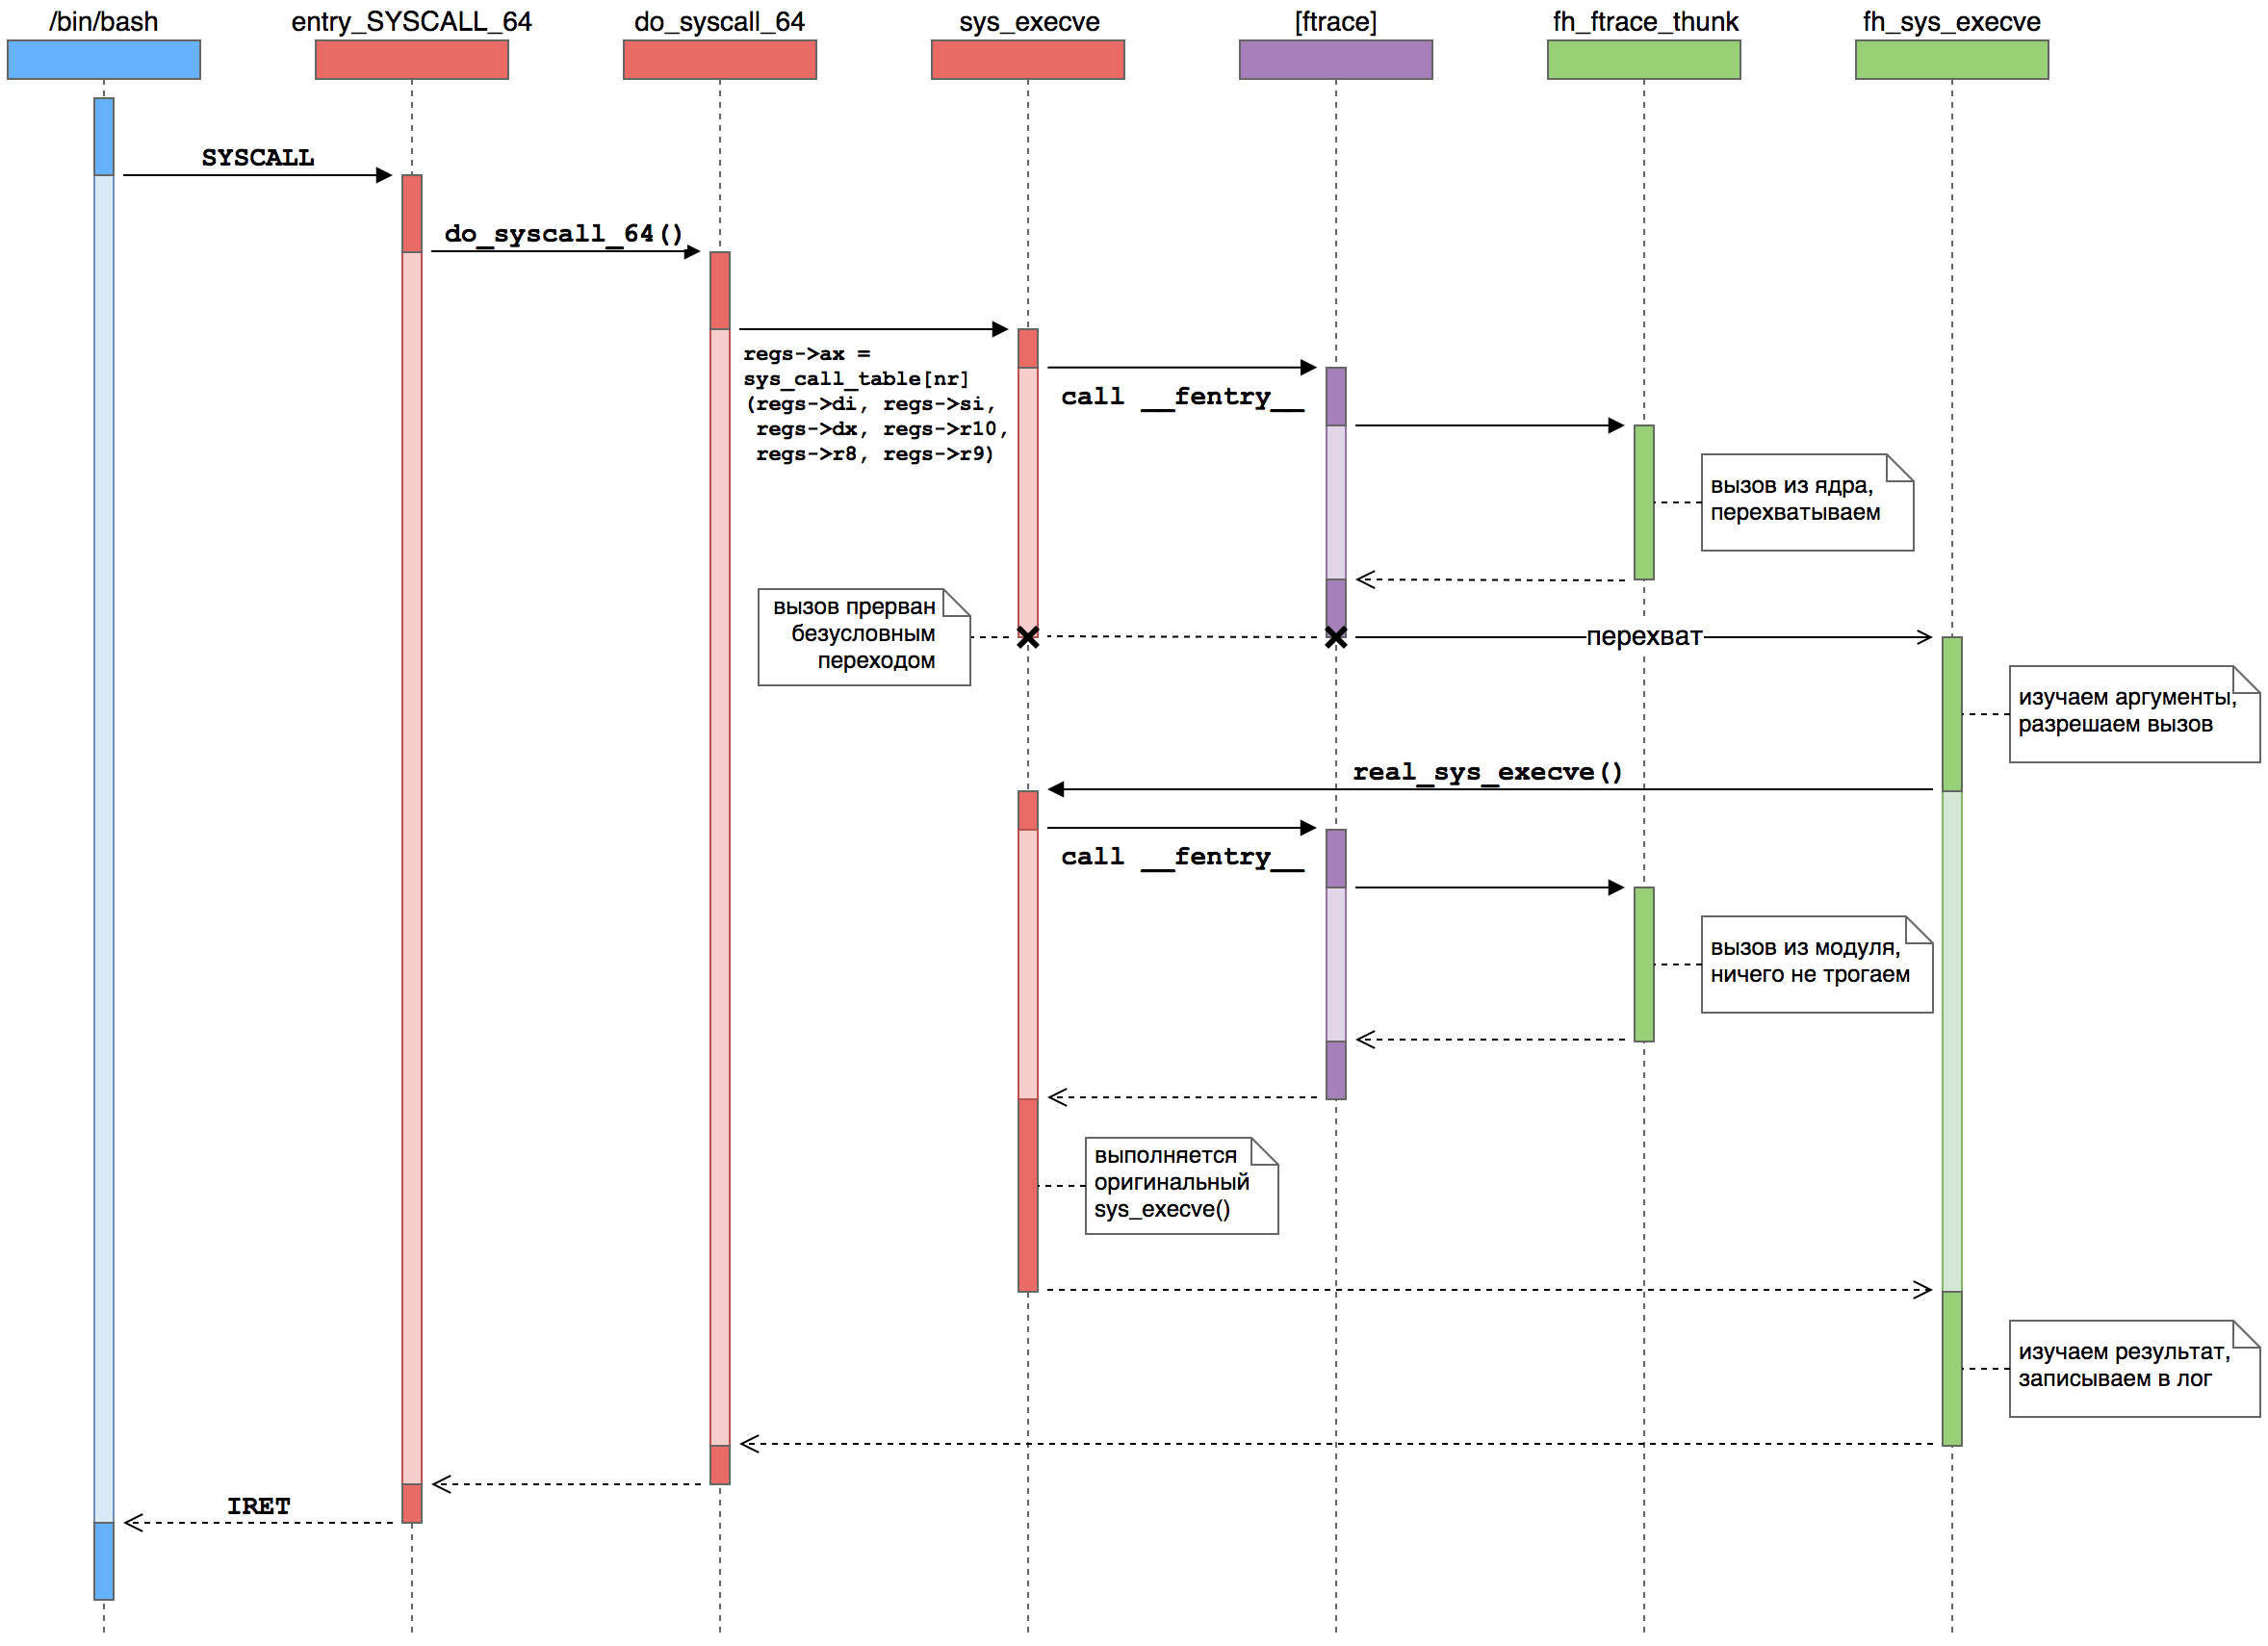
\includegraphics[width=1.0\textwidth]{img/hook_work_scheme.png}
	\caption{Алгоритм работы функции-перехватчика}
	\label{fig:spire00}
\end{figure}

\newpage
\section{Сервер}

Сервер описывается следующими структурами:
\begin{lstlisting}[language=c++,,escapeinside={(@}{@)},caption={tcp\_server\_service}]
	// Структура, описывающая и хранящие данные о текущем соединении для каждого клиента
	struct tcp_conn_handler_data {
		struct sockaddr_in *address;
		struct socket *accept_socket;
		int thread_id;
	};
	
	// Структура, описывающая и хранящие данные о текущих соединениях для всех клиентов
	struct tcp_conn_handler {
		struct tcp_conn_handler_data *data[MAX_CONNS];
		struct task_struct *thread[MAX_CONNS];
		int tcp_conn_handler_stopped[MAX_CONNS];
	};
	
	// Структура, описывающая весь сервис
	struct tcp_server_service {
		int running;
		struct socket *listen_socket;
		struct task_struct *thread;	
		struct task_struct *accept_thread;
	};
\end{lstlisting}

\section{Установка модуля}

Для компиляции реализованного модуля ядра необходимо запустить
make-файл командой \textit{make}. Make файл показан в листинге \ref{make}

\begin{lstlisting}[,,escapeinside={(@}{@)},caption={Makefile},label={make}]
KERNEL_PATH ?= /lib/modules/$(shell uname -r)/build

obj-m += kern_monitor.o

all:
	make -C $(KERNEL_PATH) M=$(PWD) modules
clean:
	make -C $(KERNEL_PATH) M=$(PWD) clean
\end{lstlisting}

%%% Local Variables:
%%% mode: latex
%%% TeX-master: "rpz"
%%% End:
